% vortex.tex
% see p18 of 2001/1 workbook 20-feb-2001
\section{A section of an ideal compressible-flow vortex}
\label{vortex-sec}
%
This flow example was used by Ian Johnston in his thesis 
and it comes with an analytic solution\,\cite{aftosmis_etal_1995a}.
With respect to \texttt{Eilmer3}, it illustrates the use of a specified flow profile as an input
and it shows the use of profile extraction, again.

The flow domain (Fig.\,\ref{vortex-geometry-fig}) includes only part of 
the first quadrant of an ideal vortex flow in inviscid air 
with $R=287$J/kg$\cdot$K, $\gamma$=1.4).
The NORTH and SOUTH boundaries are specified as reflecting walls
at radii $r_o$ and $r_i$, representing the outer and inner radii of the
vortex segment that is centred at node A.
The WEST boundary has the specified inflow as a function of radius
\begin{eqnarray}
   \rho(r) & = & \rho_i \left[
             1 + \frac{\gamma - 1}{2} M_i^2 
             \left\{ 1 - \left( \frac{r_i}{r} \right)^2 \right\}
             \right]^\frac{1}{\gamma - 1} ~~, \nonumber\\
   p(r) & = & p_i \left( \frac{\rho}{\rho_i} \right)^{\gamma} ~~, \nonumber \\
   u(r) & = & u_i \frac{r_i}{r} ~~, \nonumber
\end{eqnarray}
with $r_o = 1.384 r_i$ and the properties at the inner radius being
$M_i = 2.25$, $\rho_i = 1.0$\,kg/m$^3$ and $p_i = 100$\,kPa.

\begin{figure}[htbp]
\begin{center}
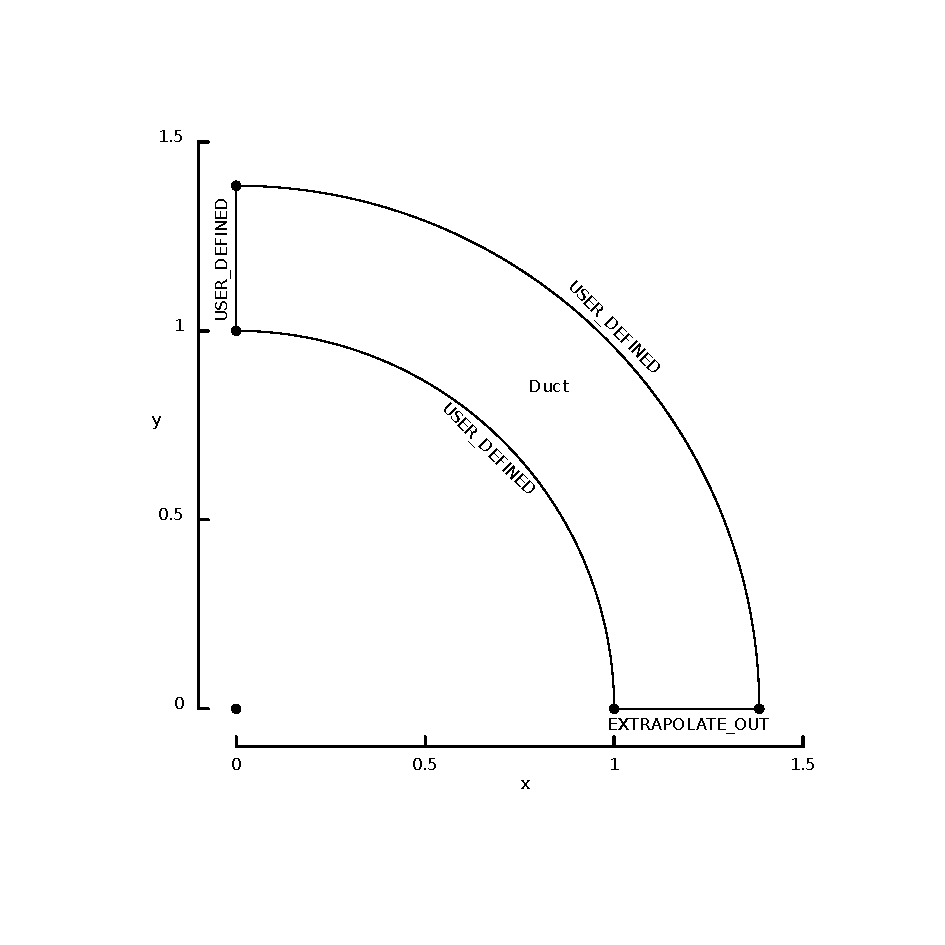
\includegraphics[width=9cm, viewport=71 74 392 392]{../2D/vortex/vtx-layout.pdf}
\end{center}
\caption{Schematic diagram of the first quadrant domain for 
         the compressible-flow vortex.}
\label{vortex-geometry-fig}
\end{figure}

Figure \ref{vortex-radial-fig} shows the radial distributions of flow properties 
and highlight some of the problems with 
the crude reflecting-wall boundary condition.
Other than at the boundaries, there is close agreement between the analytic
and numerical solutions.
The errors at the inner and outer radii stand out clearly because we
know that the trends of the flow property variations should continue
at these boundaries and not mirror what is just inside the flow domain.

\begin{figure}[htbp]
\begin{center}
\mbox{
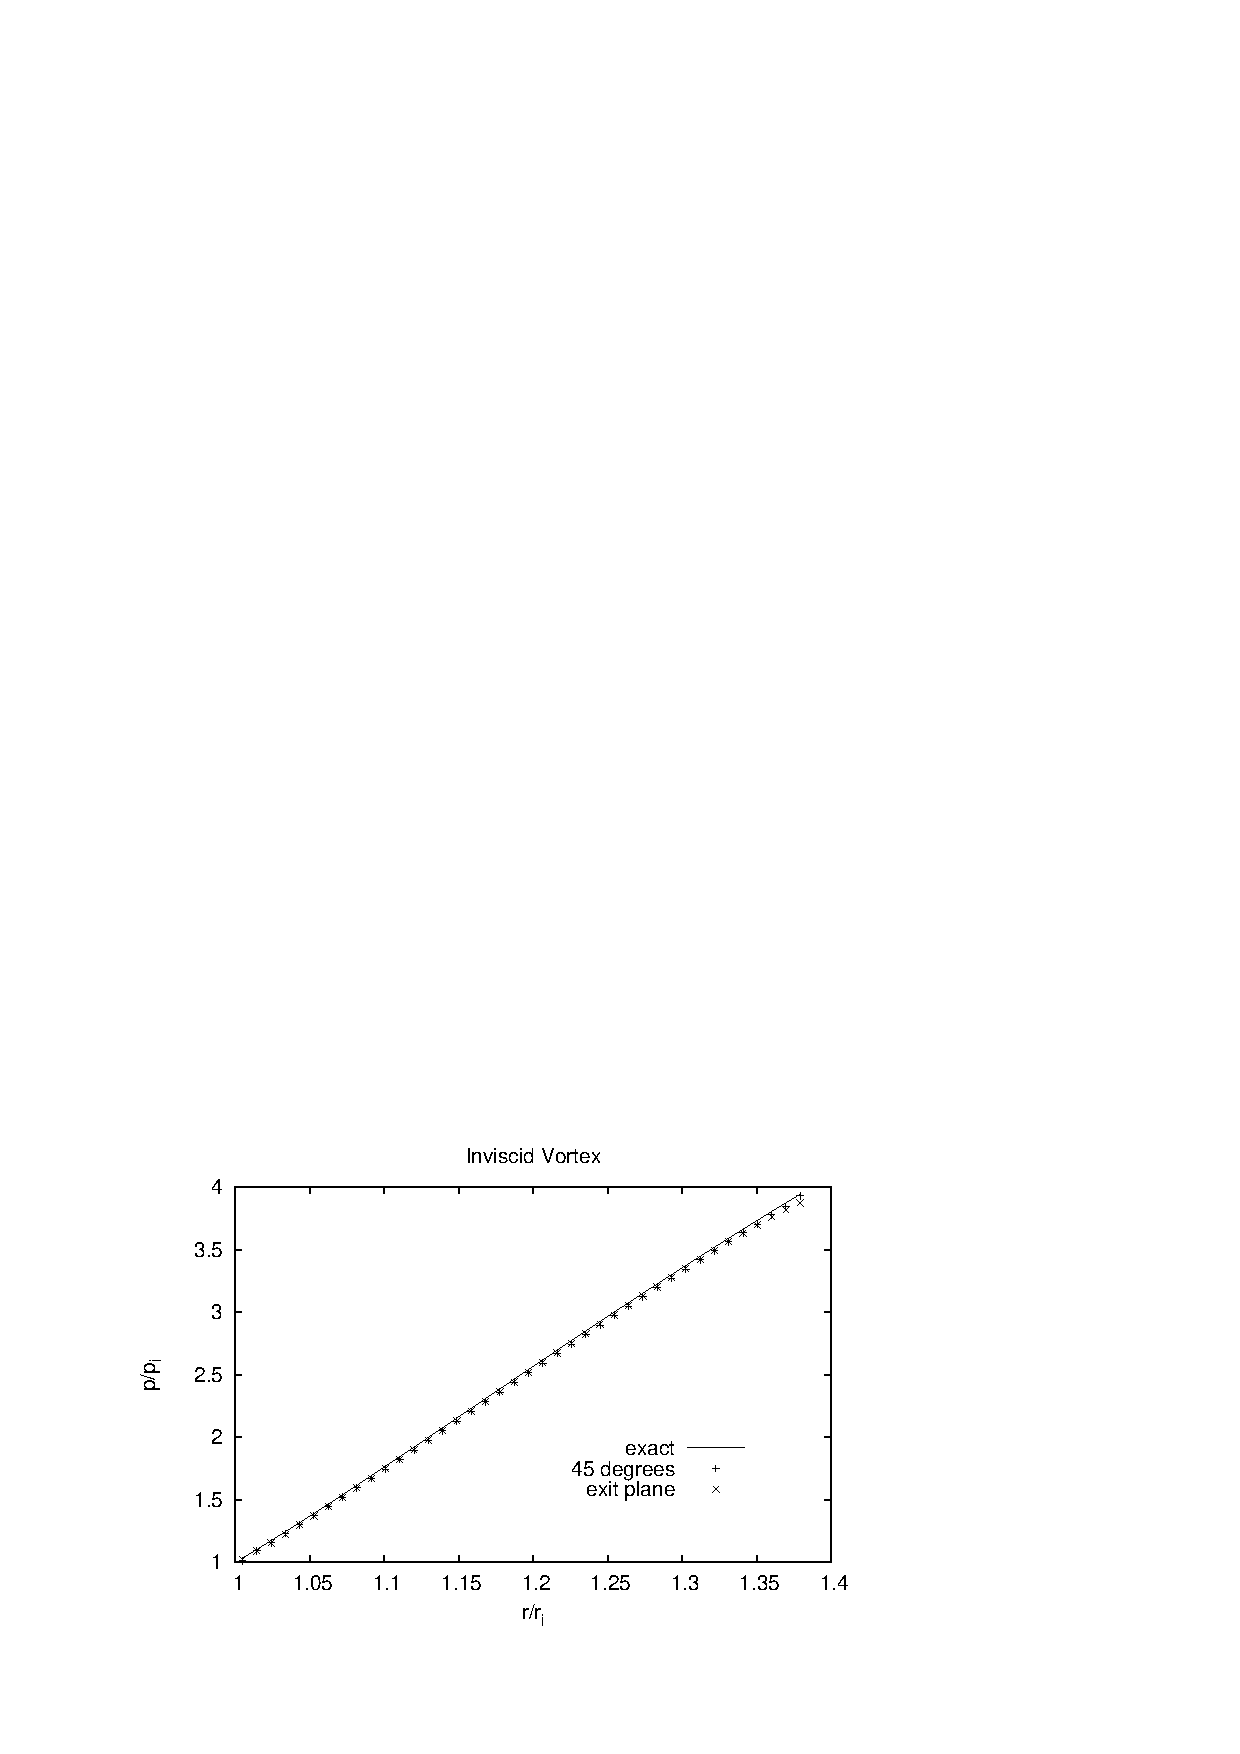
\includegraphics[width=0.5\textwidth,viewport=66 60 408 292,clip=true]{../2D/vortex/radial_profile_p.pdf}
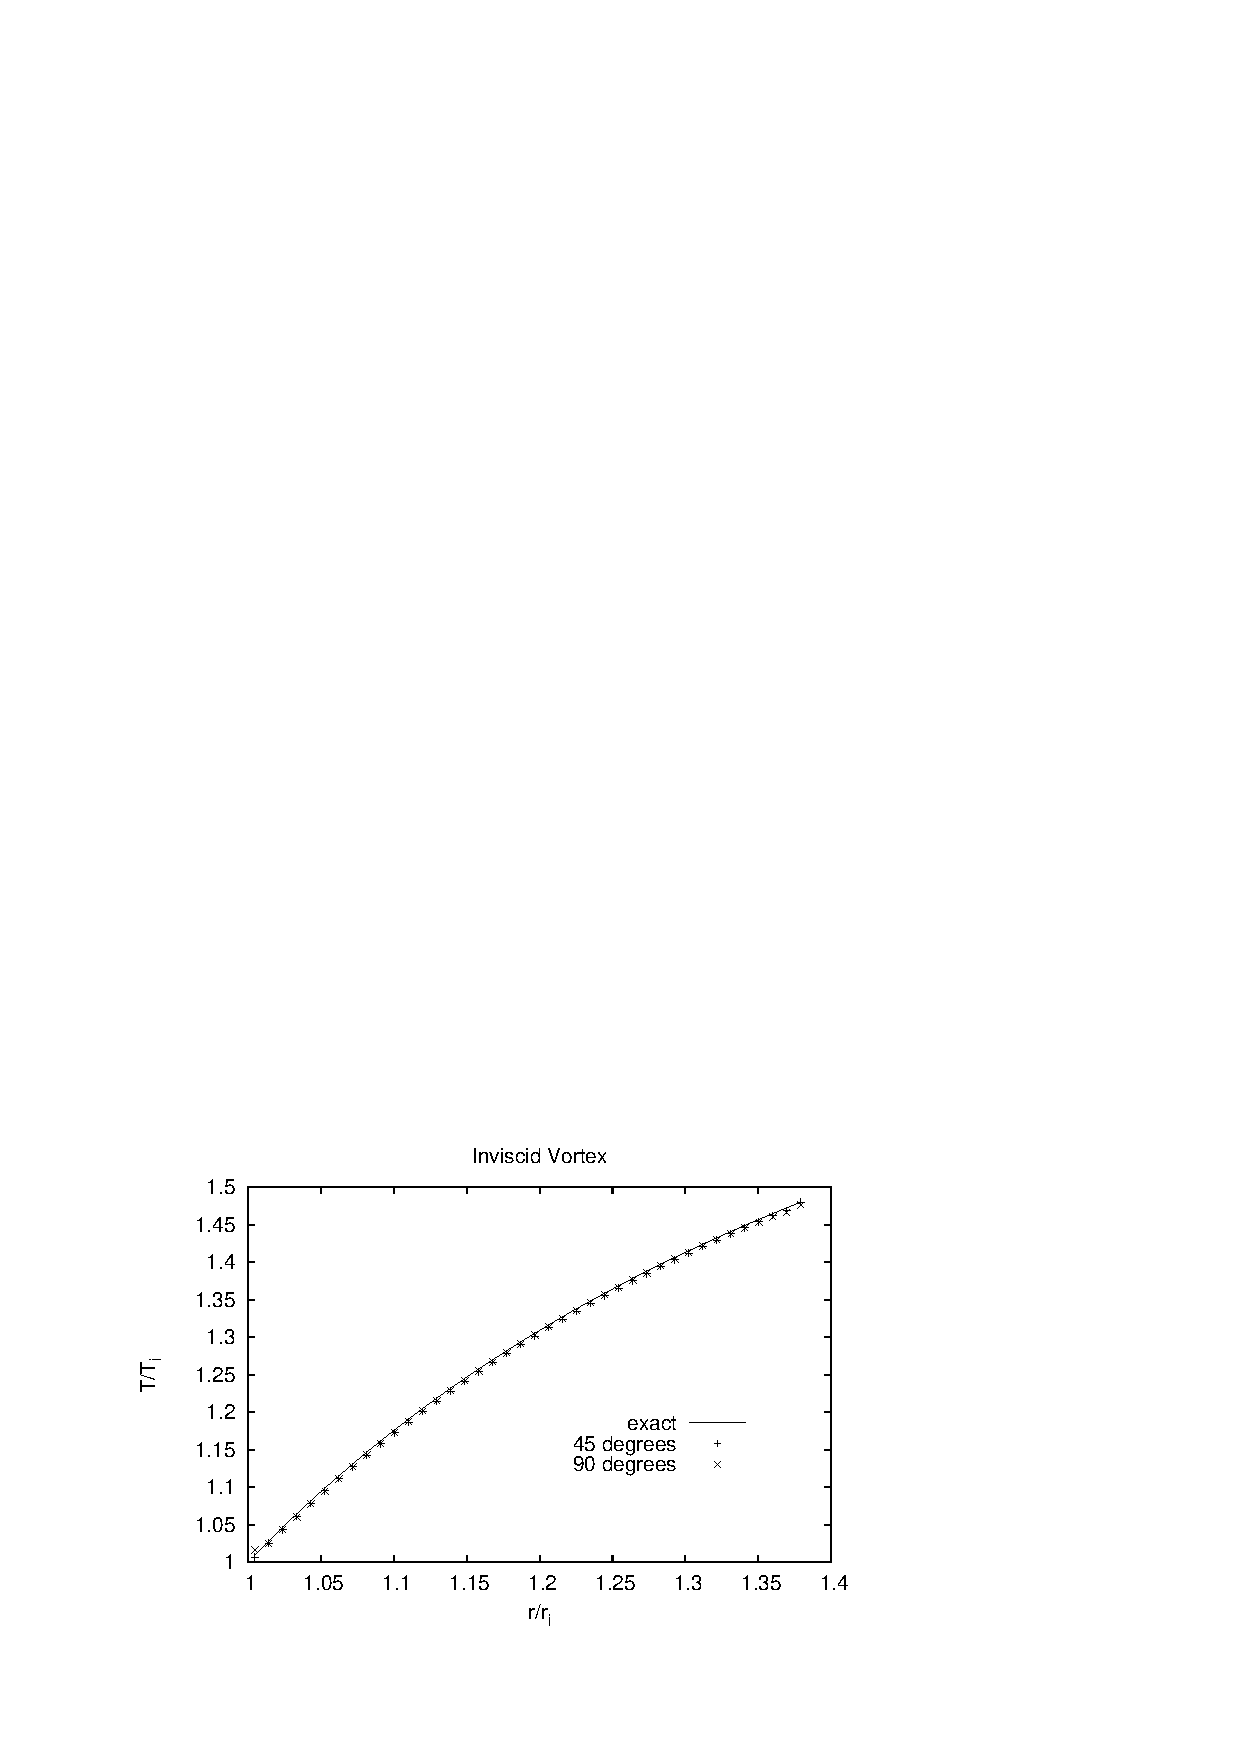
\includegraphics[width=0.5\textwidth,viewport=66 60 408 292,clip=true]{../2D/vortex/radial_profile_T.pdf}
}
\mbox{
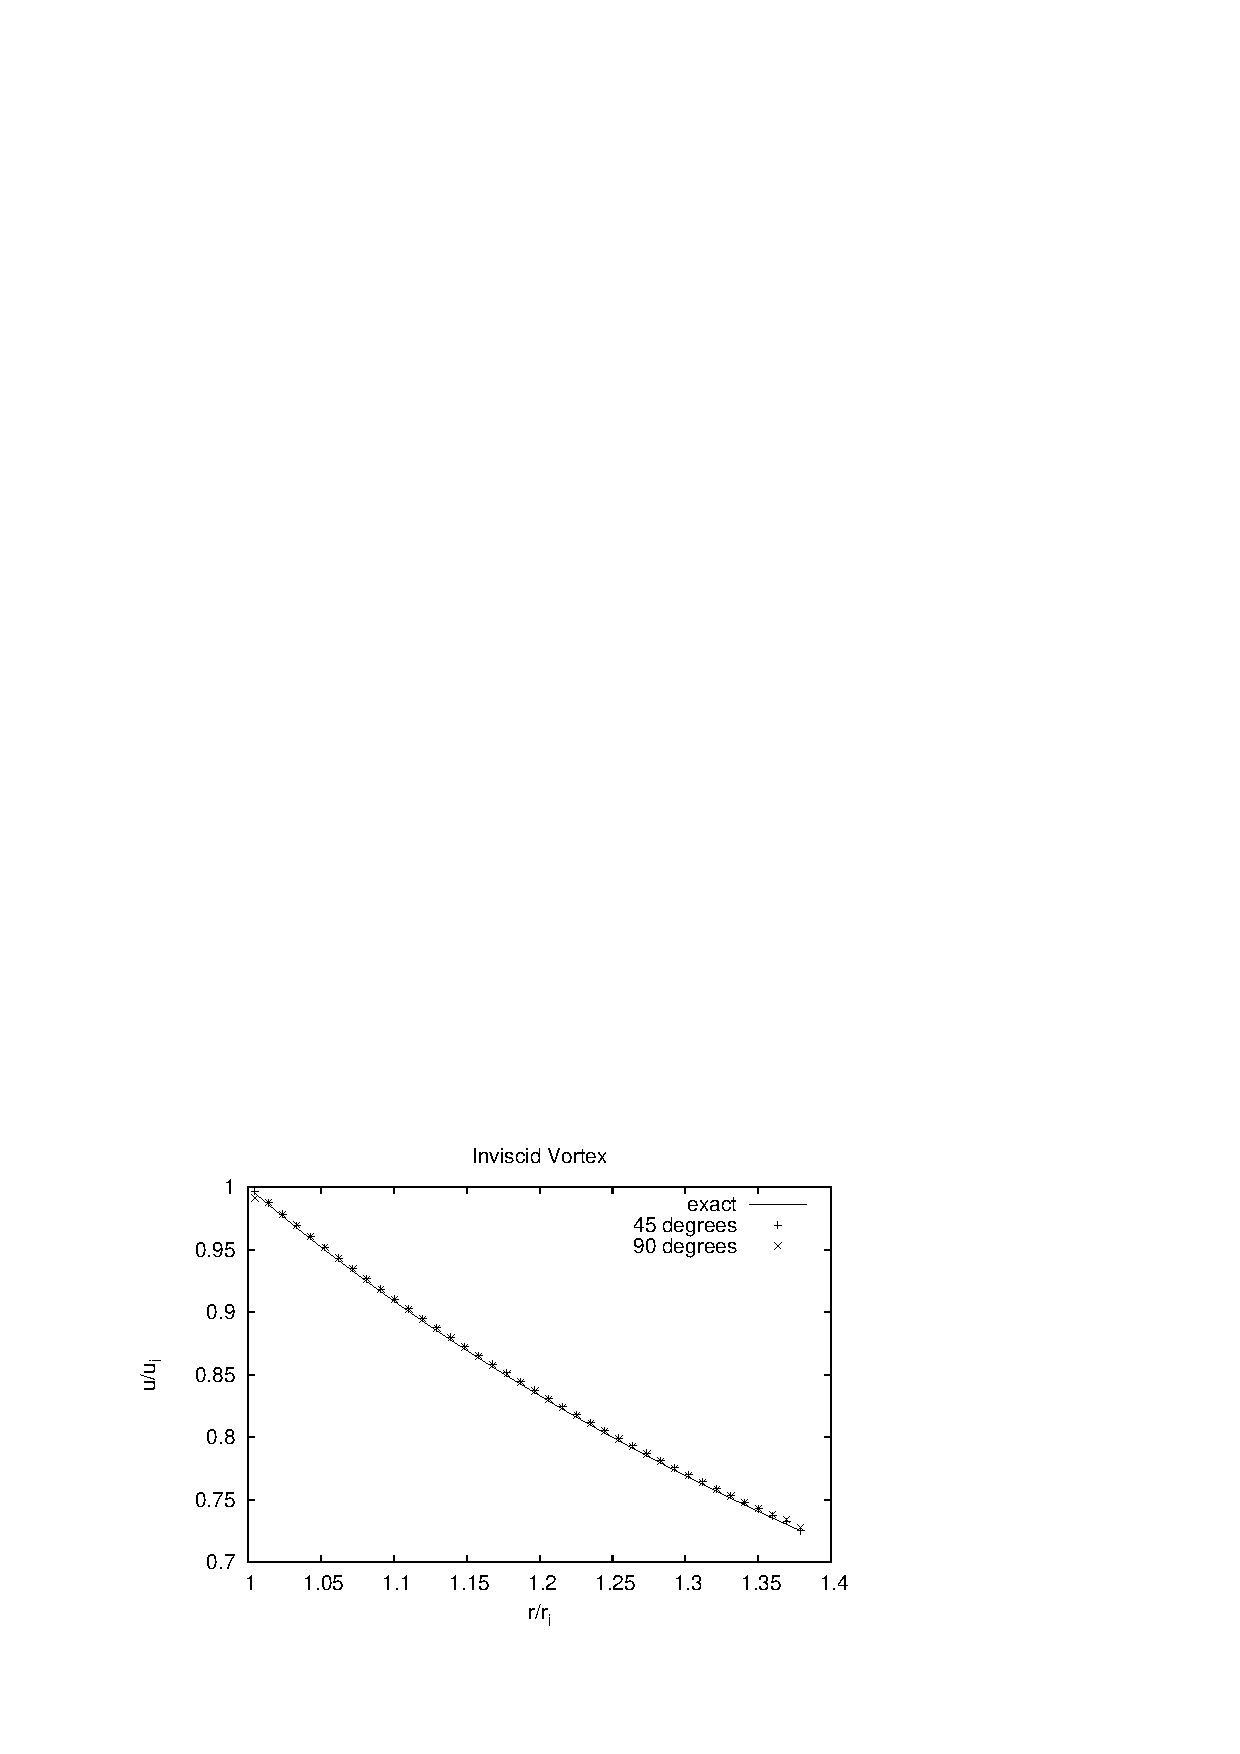
\includegraphics[width=0.5\textwidth,viewport=66 60 408 292,clip=true]{../2D/vortex/radial_profile_u.pdf}
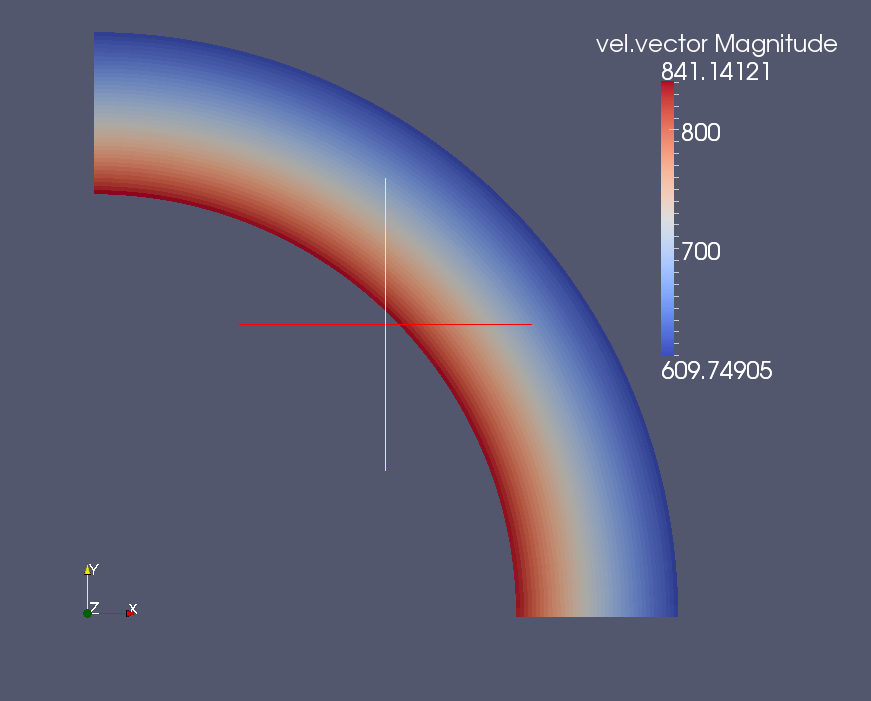
\includegraphics[width=0.5\textwidth]{../2D/vortex/vtx-speed-field.png}
}
\end{center}
\caption{Radial distributions of normalized pressure, temperature and velocity. 
  Also, the bottom right image shows the flow speed over the simulated domain}
\label{vortex-radial-fig}
\end{figure}


\newpage
\subsection{Input script (.py)}
\topbar
\lstinputlisting[language={}]{../2D/vortex/vtx.py}
\bottombar

\subsection{Boundary condition file (.lua)}
\topbar
\lstinputlisting[language={}]{../2D/vortex/udf-vortex-flow.lua}
\bottombar

\subsection{Shell scripts}
\label{vortex-sh-files}
\topbar
\lstinputlisting[language={}]{../2D/vortex/vtx_run.sh}
\bottombar

\noindent
\topbar
\lstinputlisting[language={}]{../2D/vortex/vtx_plot.sh}
\bottombar

\subsection{Notes}
\begin{itemize}
\item This simulation reaches a final time of 20\,ms in 2610 steps and,
      on an Intel Core 2 Duo CPU (E8400 @ 3.0\,Ghz) system, this takes 2\,min, 23\,s.
\item The plots were generated via the following scripts\\
      \topbarshort
      \lstinputlisting[language={}]{../2D/vortex/extract_radial.awk}
      \bottombarshort\\
      \topbarshort
      \lstinputlisting[language={}]{../2D/vortex/radial_profile.gnu}
      \bottombarshort\\
      \topbarshort
      \lstinputlisting[language={}]{../2D/vortex/make_profile.awk}
      \bottombarshort
\end{itemize}
